\documentclass[12pt,a4paper]{article}
\usepackage[utf8]{inputenc}
\usepackage[czech]{babel}
\usepackage[T1]{fontenc}
\usepackage{amsmath}
\usepackage{amsfonts}
\usepackage{amssymb}
\usepackage{graphicx}
\usepackage{mathtools}
\usepackage{fancyhdr}
\usepackage{epstopdf}
\usepackage{float}
\usepackage{gensymb}
\usepackage[final]{pdfpages}
\renewcommand{\arraystretch}{1.5}
\renewcommand{\baselinestretch}{1.25}

\title{Automatické řízení \\
	Semestrální práce}
\usepackage[top=25mm, left=35mm, right=25mm, bottom=25mm]{geometry}
\author{Miroslav Bulka, Jan Cibulka}
\date{81.121.1025}	
\setlength{\parskip}{10pt}
\begin{document}
\maketitle

\begin{figure}[h]
	\centering
	
\includegraphics[width=9cm]{obrazky/fav.png}
\end{figure}
\clearpage
\newpage


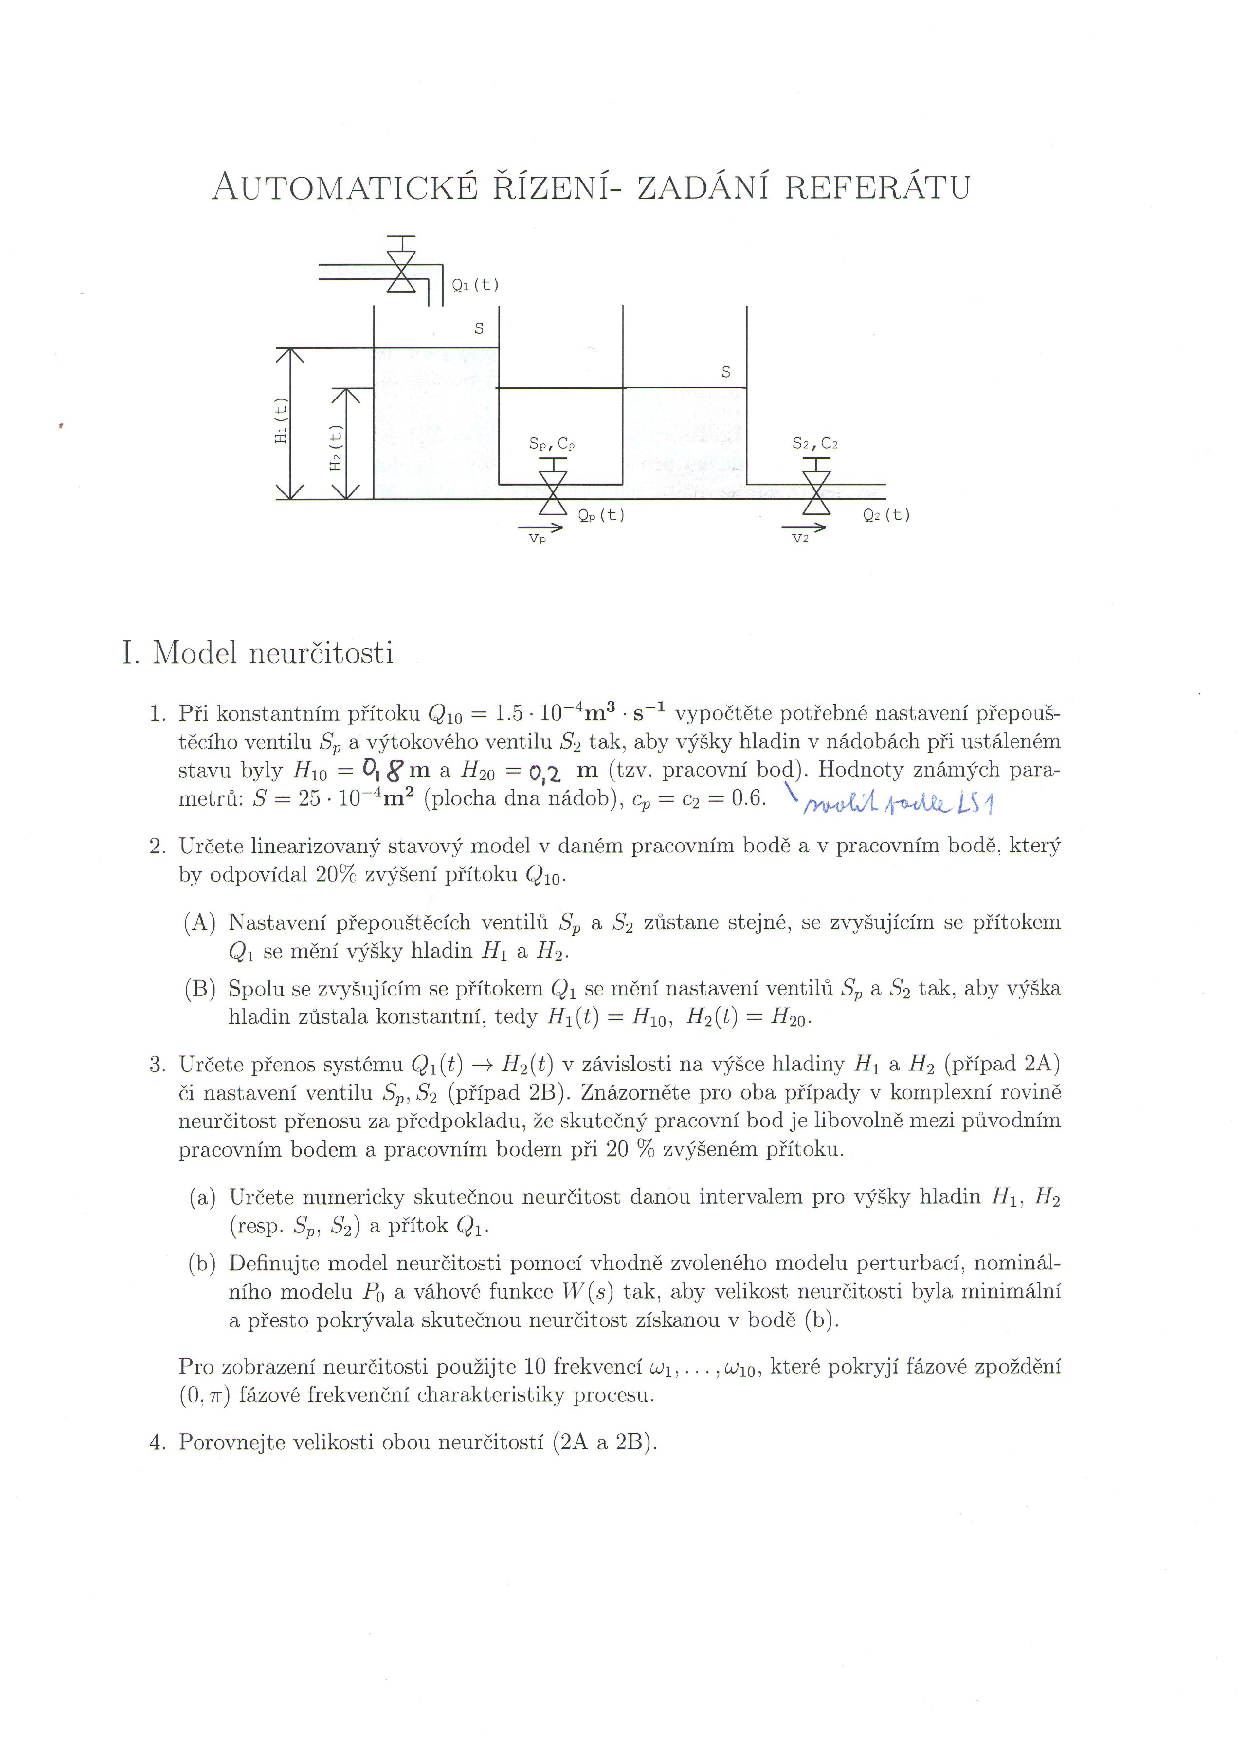
\includepdf{obrazky/Zadani1.pdf}
\newpage
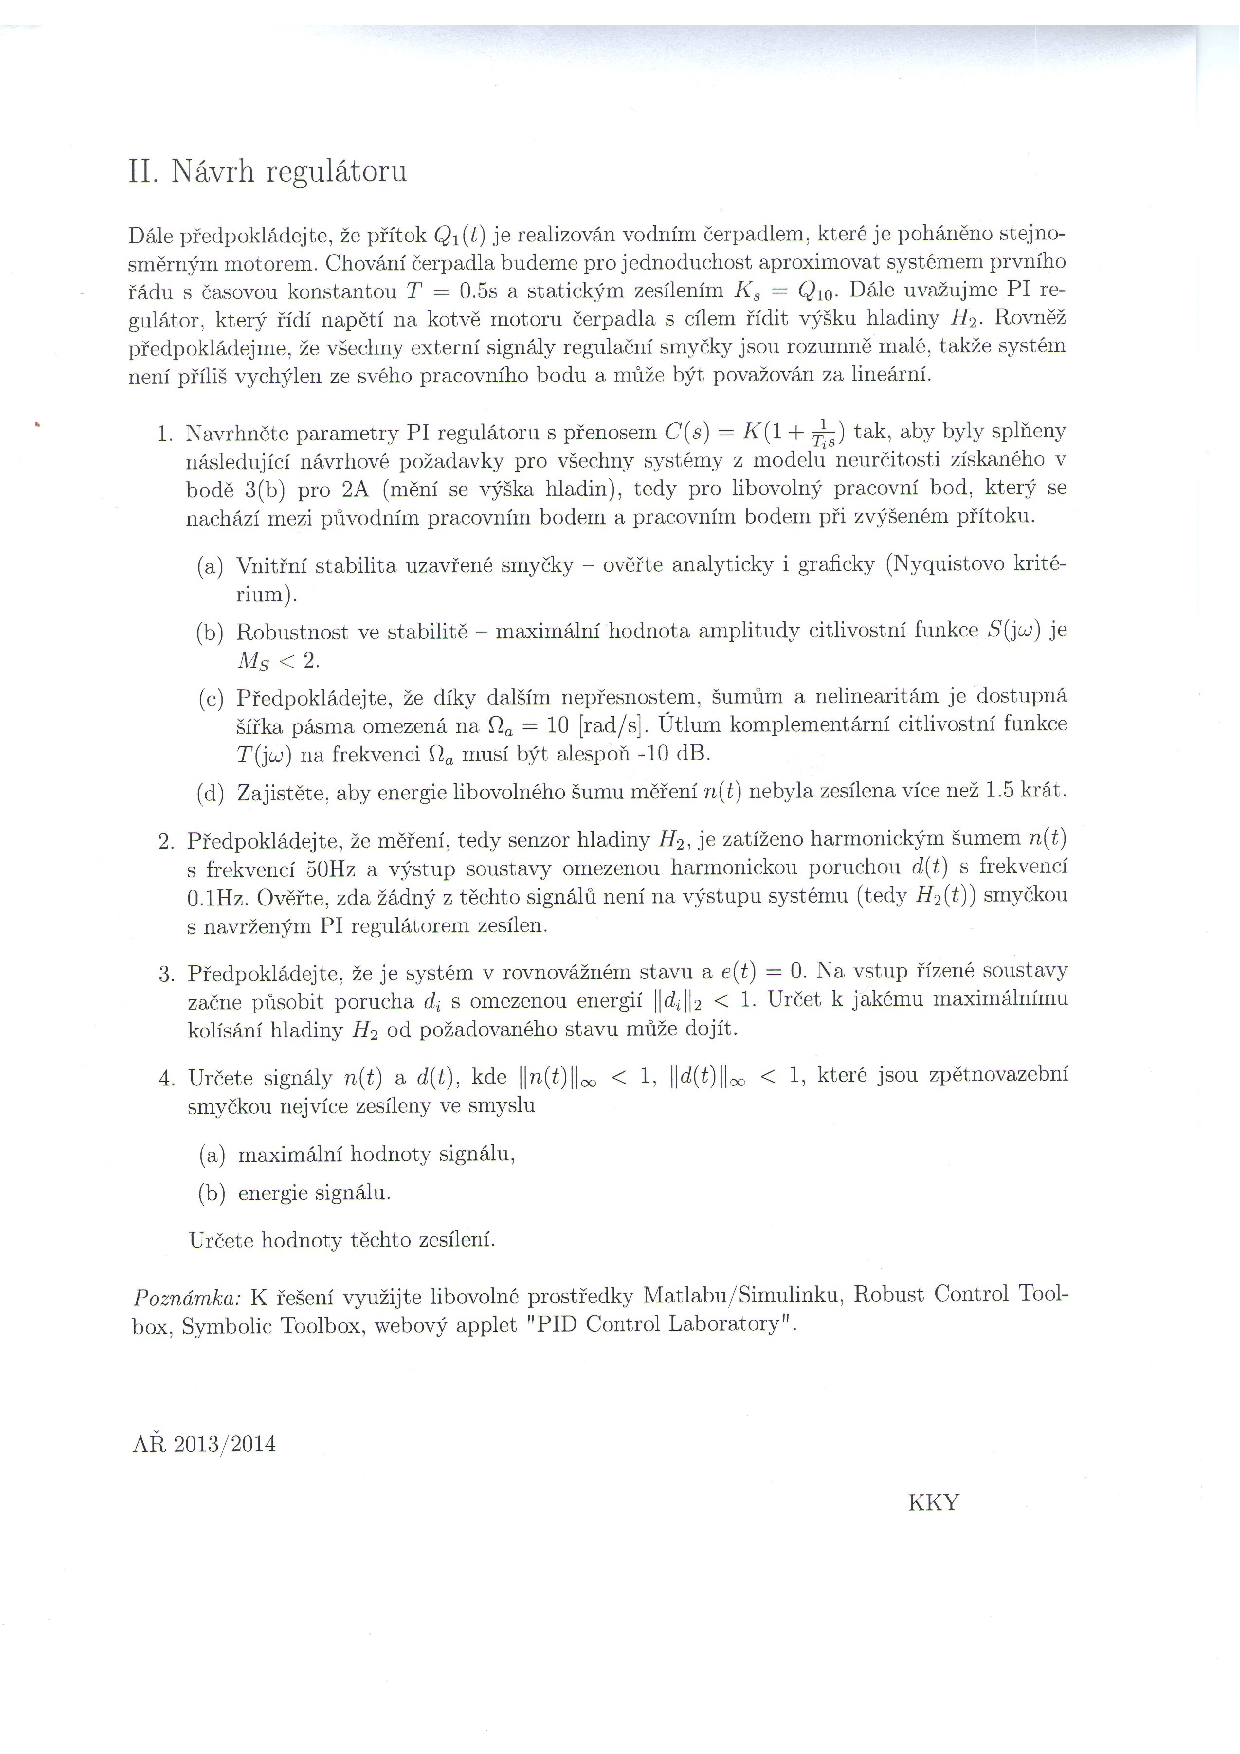
\includepdf{obrazky/Zadani2.pdf}
\newpage

\tableofcontents
\newpage

\section{Určení linearizovaného stavového modelu}
\subsection{Proměnné výšky hladin}\label{sec:2A}
Máme konstantní přítok $ Q_{1}=Q_{10}=1.5\cdot 10^{-4}m^{3}s^{-1}$, přičemž víme, že:
\begin{equation}
\left [\begin{array}{cc}
\frac{dV_{1}}{dt}\\
\frac{dV_{2}}{dt}
\end{array}\right ] = 
\left [\begin{array}{cc}
Q_{1}-Q_{p}\\
Q_{p}-Q_{2}\end{array}\right ] = 
\left [\begin{array}{cc}
Q_{1}-c_{p}S_{p}v_{p}\\
c_{p}S_{p}v_{p}-c_{2}S_{2}v_{2}\end{array}\right ].
\end{equation}
Z Bernoulliho zákona pak odvodíme:
\begin{equation}
\left [\begin{array}{cc}
v_{p} \\
v_{2}
\end{array}\right ] = 
\left [\begin{array}{cc}
\sqrt{2g\cdot (H_{1}-H_{2})}\\
\sqrt{2g\cdot (H_{2})}\end{array}\right ].
\end{equation}
Daný systém popisují diferenciální rovnice:
\begin{equation}
\left [\begin{array}{cc}
\frac{dH_{1}}{dt} \\
\frac{dH_{2}}{dt}
\end{array}\right ] = 
\left [\begin{array}{cc}
\frac{1}{S}\cdot Q_{1}-\frac{S_{p}C_{p}}{S}\cdot \sqrt{2g\cdot (H_{1}-H_{2})}\\
\frac{S_{p}C_{p}}{S}\cdot \sqrt{2g\cdot \left ( H_{1}-H_{2} \right )}-\frac{S_{2}C_{2}}{S}\cdot \sqrt{2g\cdot H_{2}}\end{array}\right ].
\end{equation}
Zavedením 
$ x_{1}(t)=H_{1}(t);\;$ 
$x_{2}(t)=H_{2}(t);\;$ 
$u(t)=Q_{1}(t)\; $
získáme
\begin{equation}
\left [\begin{array}{cc}
\frac{dx_{1}}{dt} \\
\frac{dx_{2}}{dt}
\end{array}\right ] = 
\left [\begin{array}{cc}
\frac{1}{S}\cdot u-\frac{S_{p}C_{p}}{S}\cdot \sqrt{2g\cdot (x_{1}- x_{2})}\\
\frac{S_{p}C_{p}}{S}\cdot \sqrt{2g\cdot \left ( x_{1}-x_{2} \right )}-\frac{S_{2}C_{2}}{S}\cdot \sqrt{2g\cdot x_{2}}\end{array}\right ].
\end{equation}
Za předpokladu neměnících se hladin $H_{1}$ a $ H_{2} $ budou obě derivace nulové. Položíme je tedy nulou a díky tomu získáme požadované nastavení přepouštěcího ventilu $S_{p}$ a výtokového ventilu $S_{2}$:
\begin{equation}
\left [\begin{array}{cc}
S_{p} \\
S_{2}
\end{array}\right ] = 
\left [\begin{array}{cc}
7.2864\cdot 10^{-5}\\
1.2620\cdot 10^{-4}\end{array}\right ].
\end{equation}


\paragraph*{Linearizace}
\paragraph{}

\section{Řešení - Model neurčitosti}
\subsection{První úkol}
Výpočet ustáleného stavu.
\subsection{Druhý úkol}
Linearizace ve dvou pracovních bodech.
\subsubsection{Konstantní průtoky - mění se hladina}
\label{sec:2A}
\subsubsection{Konstantní hladina - mění se průtoky}
\label{sec:2B}
\subsection{Třetí úkol}
Přenos systému, nquist asi, oba pracovní body, neurčitost.
\subsubsection{Určení numerické neurčitosti}
\subsubsection{Definovaní modelu s pertrubacemi, nominální model, váhová funkce}
\subsection{Čtvrtý úkol}
Porovnání neurčitostí z \ref{sec:2A} a \ref{sec:2B}.
\section{Řešení - Návrh regulátoru}
\subsection{První úkol}
Parametry PI regulatoru. Nejsem si jistej jestli tady jde o subukoly nebo jenom podminky pro jeden ukol.
\subsubsection{Vnitřní stabilita uzavřené smyčky (Nquistovo kritérium)}
\subsubsection{Robustnost ve stabilitě}
\subsubsection{Podmínka útlumu komplementrání citlivostní funkce}
\subsubsection{Energie šumu omezená.}
\subsection{Druhý úkol}
Harmonické poruchy.
\subsection{Třetí úkol}
Maximální kolísání hladiny.
\subsection{Čtvrtý úkol}
Určení hodnoty nějakých signálů.


\end{document}      
